\documentclass[11pt]{article}

\oddsidemargin=0in
\evensidemargin=0in
\textwidth=6.3in
\topmargin=-0.5in
\textheight=9in

\parindent=0in
%\pagestyle{empty}



%------------------------------------------------------------------
% PROBLEM, PART, AND POINT COUNTING...

% Create the problem number counter.  Initialize to zero.
\newcounter{problemnum}

% Specify that problems should be labeled with arabic numerals.
\renewcommand{\theproblemnum}{\arabic{problemnum}}


% Create the part-within-a-problem counter, "within" the problem counter.
% This counter resets to zero automatically every time the PROBLEMNUM counter
% is incremented.
\newcounter{partnum}[problemnum]

% Specify that parts should be labeled with lowercase letters.
\renewcommand{\thepartnum}{\arabic{problemnum}.\arabic{partnum}}

% Make a counter to keep track of total points assigned to problems...
\newcounter{totalpoints}

% Make counters to keep track of points for parts...
\newcounter{curprobpts}		% Points assigned for the problem as a whole.
\newcounter{totalparts}		% Total points assigned to the various parts.

% Make a counter to keep track of the number of points on each page...
\newcounter{pagepoints}
% This counter is reset each time a page is printed.

% This "program" keeps track of how many points appear on each page, so that
% the total can be printed on the page itself.  Points are added to the total
% for a page when the PART (not the problem) they are assigned to is specified.
% When a problem without parts appears, the PAGEPOINTS are incremented directly
% from the problem as a whole (CURPROBPTS).


%---------------------------------------------------------------------------


% The \problem environment first checks the information about the previous
% problem.  If no parts appeared (or if they were all assigned zero points,
% then it increments TOTALPOINTS directly from CURPROBPTS, the points assigned
% to the last problem as a whole.  If the last problem did contain parts, it
% checks to make sure that their point values total up to the correct sum.
% It then puts the problem number on the page, along with the points assigned
% to it.

\newenvironment{problem}[1]{
% STATEMENTS TO BE EXECUTED WHEN A NEW PROBLEM IS BEGUN:
%
% Increment the problem number counter, and set the current \ref value to that
% number.
\refstepcounter{problemnum}
%
% Add some vspace to separate from the last problem.
\vspace{0.15in} \par
%
\setcounter{curprobpts}{#1} \setcounter{totalparts}{0}	% Reset counters.
%
% Now put in the "announcement" on the page.
{\Large \bf \theproblemnum. \normalsize ({\it \arabic{curprobpts} point\null\ifnum \value{curprobpts} = 1\else s\fi}\/)}
}{
% STATEMENTS TO BE EXECUTED WHEN AN OLD PROBLEM IS ENDED:
%
% If no parts to problem, then increment TOTALPOINTS and PAGEPOINTS for the
% entire problem at once.
\ifnum \value{totalparts} = 0
	\addtocounter{totalpoints}{\value{curprobpts}}	% Add pts to total.
	\addtocounter{pagepoints}{\value{curprobpts}}	% Add pts to page total.
%
% If there were parts for the problem, then check to make sure they total up
% to the same number of points that the problem is worth. Issue a warning
% if not.
\else \ifnum \value{totalparts} = \value{curprobpts}
	\else \typeout{}
	\typeout{!!!!!!!   POINT ACCOUNTING ERROR   !!!!!!!!}
	\typeout{PROBLEM [\theproblemnum] WAS ALLOCATED \arabic{curprobpts} POINTS,}
	\typeout{BUT CONTAINS PARTS TOTALLING \arabic{totalparts} POINTS!}
	\typeout{}
	\fi
\fi
}


%---------------------------------------------------------------------------


% The \newpart command increments the part counter and displays an appropriate
% lowercase letter to mark the part.  It adds points to the point counter
% immediately.  If 0 points are specified, no point announcement is made.
% Otherwise, the announcement is in scriptsize italics.

\newcommand{\newpart}[1]
{
\refstepcounter{partnum}	% Set the current \ref value to the part number.
%\hspace{0.0in}		% Indent the part by a quarter inch.
%
% If points are to be printed for this problem (signaled by point value > 0),
% then put them in in scriptsize italics.
\ifnum #1 > 0
	\makebox[0.5in][l]{{\bf \thepartnum.} {\bf ({\it #1 pt\ifnum #1 = 1\else s\fi\/}) \,\,}}
\else
	\makebox[0.25in][l]{({\bf \thepartnum})}
\fi
%
\hspace{0.1in}		% Lead the material away from the part "number".
%
\addtocounter{totalparts}{#1}	% Add points to totalparts for this problem.
\addtocounter{pagepoints}{#1}	% Add points to total for this page.
\addtocounter{totalpoints}{#1}	% Add points to total for entire test.
}


%---------------------------------------------------------------------------



% Just in case you want to skip some numbers in your test...

\newcommand{\skipproblem}[1]{\addtocounter{problemnum}{#1}}



%---------------------------------------------------------------------------


% The \showpoints command simply gives a count of the total points read in up to
% the location at which the command is placed.  Typically, one places one
% \showpoints command at the end of the latex file, just prior to the
% \end{document} command.  It can appear elsewhere, however.

\newcommand{\showpoints}
{
\typeout{}
\typeout{====> A TOTAL OF \arabic{totalpoints} POINTS WERE READ.}
\typeout{}
}


%---------------------------------------------------------------------------



\usepackage{graphicx}
\usepackage[english]{babel}
\usepackage[latin1]{inputenc}
\usepackage{times}
\usepackage[T1]{fontenc}
\usepackage{amsmath}
\usepackage{amssymb}
\usepackage{subfigure}
\usepackage{algorithmic}
\usepackage{algorithm}
\usepackage{url}

\usepackage{xr}
\externaldocument{rbm-notes}

\newcommand{\argmax}{\mathop{\arg\max}}
\newcommand{\deriv}[2]{\frac{\partial{#1}}{\partial {#2}} }
\newcommand{\dsep}{\mbox{dsep}}
\newcommand{\Pa}{\mathop{Pa}}
\newcommand{\ND}{\mbox{ND}}
\newcommand{\De}{\mbox{De}}
\newcommand{\Ch}{\mbox{Ch}}
\newcommand{\graphG}{{\mathcal{G}}}
\newcommand{\graphH}{{\mathcal{H}}}
\newcommand{\setA}{\mathcal{A}}
\newcommand{\setB}{\mathcal{B}}
\newcommand{\setS}{\mathcal{S}}
\newcommand{\setV}{\mathcal{V}}
\DeclareMathOperator*{\union}{\bigcup}
\DeclareMathOperator*{\intersection}{\bigcap}
\DeclareMathOperator*{\Val}{Val}
\newcommand{\mbf}[1]{{\mathbf{#1}}}
\newcommand{\eq}{\!=\!}
\newcommand{\cut}[1]{{}}

\begin{document}

%%%(change to appropriate class and semester)
{\centering
  \rule{6.3in}{2pt}
  \vspace{1em}
  \Large{
    CS688: Graphical Models - Spring 2018\\
    Assignment 4\\
  }
  \vspace{1em}
  Assigned: Thursday, Mar 29th. Due: Thursday, April 13th 11:59pm\\
  \vspace{0.1em}
  \rule{6.3in}{1.5pt}
}
\vspace{1pc}

\textbf{Getting Started:} You should complete the assignment using your own installation of Python 2.7. The only modules you are permitted to use in your implementations are Numpy and SciPy. To get started with the code portions of the assignment, download the assignment archive from Moodle and unzip the file. The data files for this assignment are in the \textit{data} directory. Code templates are in the \texttt{code} directory.\\

\textbf{Deliverables:} This assignment has two types of deliverables: a report and code files.

\begin{itemize}
\item \textbf{Report: } The solution report will give your answers to the homework questions. Items that you should include in your report are marked with \textbf{(report)}. The maximum length of the report is 5 pages in 11 point font, including all figures and tables. You can use any software to create your report, but your report must be submitted in PDF format. You will upload the PDF of your report to Gradescope under \verb|HW04-Report| for grading. It is strongly recommended that you typeset your report. To assist with this if you wish to use Latex, the Latex source of the handout is also included in the homework archive.

\item \textbf{Code: } The second deliverable is your code. Items that you should include in your code are marked with \textbf{(code)}.  Your code must be Python 2.7 (no iPython notebooks, other formats, or code from other versions of Python). You will upload a zip file (not rar, bz2 or other compressed format) containing all of your code to Gradescope under \verb|HW04-Programming|.  When unzipped, your zip file should produce a directory called \verb|code|. Do not upload the data directory to Gradescope.

\end{itemize}
\vspace{0.5em}

\textbf{Academic Honesty Statement:} Copying solutions from external
sources (books, web pages, etc.) or other students is considered
cheating. Sharing your solutions with other students is also
considered cheating. Collaboration indistinguishable from copying is a violation 
of the course's collaboration policy and will be treated as cheating.
Any detected cheating will result in a grade of 0
on the assignment for all students involved, and potentially a grade
of F in the course.\\

\textbf{Introduction:} In this assignment, you will experiment with Markov Chain Monte Carlo inference and stochastic maximum likelihood learning for restricted Boltzmann Machines (RBMs). A tutorial
introduction  to RBMs is provided in the accompanying notes.
We will use binary image data for this assignment taken from the MNIST handwritten digit data set. Examples from this data set are pictured below. Each image has size $28\times 28$.\\

\begin{figure}[ht]
\centering
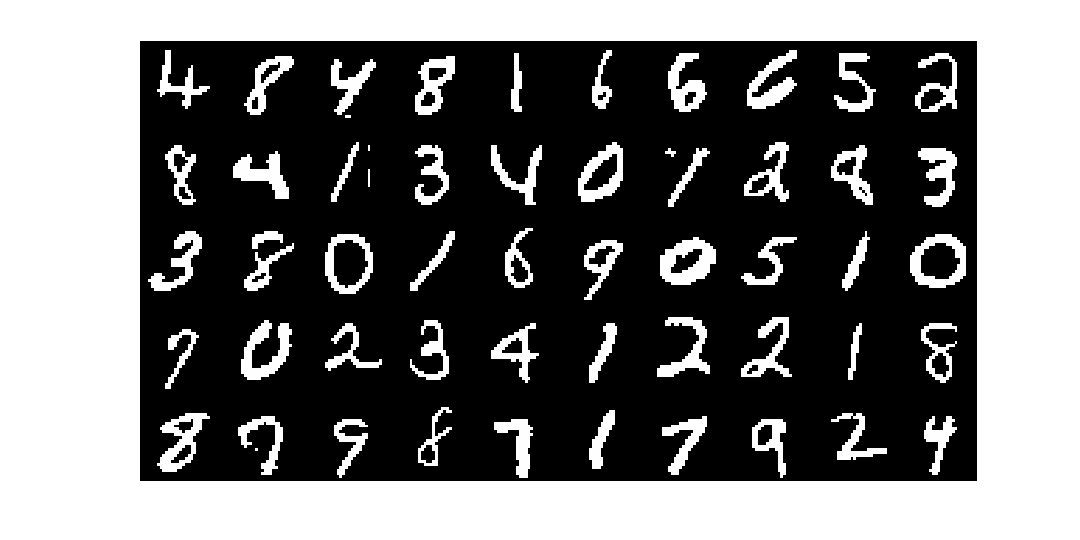
\includegraphics[width=3.1in]{Figures/example_digits.png}
\label{fig_data}
\caption{Example data from the MNIST data set.}
\end{figure}

A model trained on the MNIST data has been provided for use in inference experiments. The training data set contains $60,000$ cases and the test set contains $10,000$ cases. Each data case contains one $28\times 28$ binary image stored as a $784$ element vector.\\


\begin{problem}{20} \textbf{Derivations:} Perform the following derivations. All equation numbers refer to the accompanying RBM notes. Show your work.\\

\newpart{10} Starting from the definition of the joint probability on $\mbf{X}$ and $\mbf{H}$ given in Equation \ref{joint-prob}, derive the conditional probability  $P_W(X_d=x_d|\mbf{h})$ shown in Equation \ref{pxgh}. \textbf{Hint:} You can do this from first principles, but it will be easier if you use the factor reduction algorithm. (report)\\

\newpart{10} Starting from the definition of the average marginal log likelihood in Equation \ref{marginal_loglik}, derive the partial derivative of the average marginal log likelihood with respect to $W^P_{ij}$ shown in Equation \ref{deriv_WP}. \textbf{Hint:} This derivation is very similar to both the Ising model and CRF model maximum likelihood parameter estimation derivations (report).
\end{problem}

\begin{problem}{15} \textbf{Sampling Implementation:} Implement the components of the block Gibbs sampler described in the RBM notes in the file \verb|rbm.py|. In particular, complete the functions \verb|pxgh|, \verb|phgx|, \verb|gibbs_x_step|, \verb|gibbs_h_step|
as well as the energy function \verb|energy| and the helper functions \verb|get_parameters| and \verb|set_parameters|. 	
	 You may create any additional support functions and data structures that you need. (code)
\end{problem}

\begin{problem}{20} \textbf{Sampling with Single Chains:} In the models directory, you will find the files \textit{MNISTWP.npy}, \textit{MNISTWB.npy} and \textit{MNISTWC.npy}. These files contain the parameters of a binary RBM model trained on the MNIST data set using $K=100$ hidden units. $W^P$ is a $784 \times 100$ array,
$W^B$ is a $1\times 100$ array, and $W^C$ is a $1\times 784$ array. Use your implementation  to answer the following questions. Add your code to \verb|experiment.py|\\

\newpart{5}  Run the Gibbs sampler on the trained MNIST model for $500$ iterations using the first training data case as the first sample $\tilde{\mbf{x}}_1$. Display the last 100 samples from the chain as $28 \times 28$ images and include these images in your report (there is helper code for assembling the individual images into a single large image in \verb|util.py|). (report)\\

\newpart{5}   Now, compute the joint energy $e_s = E_W(\tilde{\mbf{x}}_s,\tilde{\mbf{h}}_s)$ for each sampled $(\tilde{\mbf{x}}_s,\tilde{\mbf{h}}_s)$ pair using Equation \ref{energy} and provide a line plot showing energy versus sample index for all samples. Based on this plot, indicate what you think a reasonable burn-in time would be. (report)\\

\newpart{5}  Next, discard the samples from before your selected burn-in period
and compute the autocorrelation of the remaining sequence of $e_s$ values (there is
code in \verb|util.py| for computing autocorrelations). Plot the autocorrelation 
values as a line graph and include the graph in your report. (report)\\

\newpart{5} Based only on the evidence obtained in parts 3.1 to 3.3, what would you conclude about how efficiently the block Gibbs sampler is traversing the state space? 
\end{problem}

\begin{problem}{20} \textbf{Sampling with Multiple Chains:} Use your implementation of the Block Gibbs sampler and the trained parameters (as described in Question 2) to answer the following questions.\\

\newpart{5}  Use your implementation to run $100$ separate chains for $500$ iterations each. Initialize the $i^{th}$ chain so that
its first sample of $\tilde{\mbf{x}}_1$ is the $i^{th}$ training case. Display the final sample of the visible variables from each of the $100$ chains as a set of $28 \times 28$ images and include the result in your report. (report) \\

\newpart{5} For the first $5$ of the $100$ chains run in 4.1, compute the energy of each sample of the visible and hidden variables $(\tilde{\mbf{x}}_{s},\tilde{\mbf{h}}_{s})$ using Equation \ref{energy}. Plot a single graph with $5$ curves showing the energy trace for each chain versus the sampling iteration. (report)\\

\newpart{5} Based on this additional evidence, what can you conclude about burn-in time time and how efficiently the block Gibbs sampler is traversing the state space? (report) \\

\newpart{5} Running multiple Gibbs chains can be expensive; however, the computations required are completely independent for each cain. Provide Python/Numpy code showing how both the \verb|gibbs_x_step|   and \verb|gibbs_h_step|  algorithms can be computed for $C$ chains using only Numpy operations and no Python for loops. Assume the input to \verb|gibbs_x_step|  is a $C\times K$ array of hidden states, and the output should be a $C\times D$ array of sampled visible states. Similarly, assume that the input to  \verb|gibbs_h_step| is a $C\times D$ array of visible states, and the output should be a
$C\times K$ array of sampled hidden states. This is referred to as code \textit{vectorization}. Since numpy is written in C and supports multi-core parallelism, such an implementation will be much faster than an implementation using Python for loops. \textbf{Hint:} The entire implementation of each function requires two lines of code. (report)

\end{problem}

\begin{problem}{15} \textbf{Learning Implementation:} Implement regularized mini batch stochastic gradient ascent for learning the RBM model, as described in the RBM notes. In particular, implement the functions \verb|grad| and \verb|fit| in \verb|rbm.py|. If you find that your implementation is slow, use your vectorized implementation for sampling. The gradient computations can also be fully
vectorized, which can significantly accelerate your code. (code)
\end{problem}
	
\begin{problem}{10} \textbf{Learning Experiments:} Use your RBM implementation to answer the following questions. If you find that your implementation is slow, use your vectorized implementation for sampling. The gradient computations can also be fully vectorized, which can significantly accelerate your code. \\

\newpart{5}  Run your learning algorithm on the MNIST training data using $K=400$ hidden units. Keep the other
parameters of \verb|fit| at their defaults. When training is complete, display the final sample from each of the $100$ Gibbs chains as a $28\times 28$ image and include the result in your report. (report)\\

\newpart{5} The samples drawn from an RBM can be fairly noisy. A common alternative to displaying the sampled value $\tilde{\mbf{x}}_s$
when the data represent binary images is to display an image where the value of each pixel is the probability that the pixel value should be $1$. Thus, instead of displaying an image based on $\tilde{x}_{ds}$, the image is based on the values $p_{ds} = P(X_d=1|\mbf{H}=\tilde{\mbf{h}}_{s-1})$. Produce a second set of $100$ images visualizing the final state of the chain from part 6.1 
in terms of the values $p_{ds}$ for each of the 100 chains and include this image in your report. \textbf{Hint:} Consider the second output of \verb|gibbs_x_step|. (report) 

\end{problem}

\showpoints
\end{document} 